\documentclass[12pt]{article}
\usepackage[utf8]{inputenc}
\usepackage[T1]{fontenc}
\usepackage{amsmath}
\usepackage{amsfonts}
\usepackage{amssymb}
\usepackage[version=4]{mhchem}
\usepackage{stmaryrd}
\usepackage{bbold}
\usepackage{graphicx}
\usepackage{subcaption}
\usepackage[export]{adjustbox}
\usepackage[a4paper, left=0.25in, right=0.25in, top=1in, bottom=1in]{geometry}
\graphicspath{ {./images/} }

\title{Assignment 4: Simulations with MPS }


\author{Instructor: Lesik Motrunich\\
TA: Liam O'Brien}
\date{}


%New command to display footnote whose markers will always be hidden
\let\svthefootnote\thefootnote
\newcommand\blfootnotetext[1]{%
  \let\thefootnote\relax\footnote{#1}%
  \addtocounter{footnote}{-1}%
  \let\thefootnote\svthefootnote%
}

%Overriding the \footnotetext command to hide the marker if its value is `0`
\let\svfootnotetext\footnotetext
\renewcommand\footnotetext[2][?]{%
  \if\relax#1\relax%
    \ifnum\value{footnote}=0\blfootnotetext{#2}\else\svfootnotetext{#2}\fi%
  \else%
    \if?#1\ifnum\value{footnote}=0\blfootnotetext{#2}\else\svfootnotetext{#2}\fi%
    \else\svfootnotetext[#1]{#2}\fi%
  \fi
}

\begin{document}
\maketitle
Due: $4 \mathrm{pm}$ Thursday, May 28,2024



\section*{4 Assignment: MPS simulations using TEBD}
We will again study the quantum Ising model subject to a magnetic field with both transverse and longitudinal components:


\begin{equation*}
H=-J \sum_{j=1}^{L-1} \sigma_{j}^{z} \sigma_{j+1}^{z}-h^{x} \sum_{j=1}^{L} \sigma_{j}^{x}-h^{z} \sum_{j=1}^{L} \sigma_{j}^{z} \tag{15}
\end{equation*}


Set $J=1$ and the magnetic field to $\left(h^{x}, h^{z}\right)=(-1.05,0.5)$, the same values as in Assignment 3, to allow you to test your MPS-based approach against exact diagonalization for small system sizes. Because we are now working with MPS, consider the system with open boundary conditions where the MPS simulations are most transparent. To specify a time-evolution procedure, this Hamiltonian can be arranged into three groups of commuting terms (i.e., commuting within each group): $H=H_{\text {odd }}+H_{\text {even }}+H_{\text {field }}$, each of which can be readily exponentiated. The groupings are


\begin{align*}
& H_{\mathrm{odd}}=-J \sum_{j=1,3,5, \ldots} \sigma_{j}^{z} \sigma_{j+1}^{z}=-J\left(\sigma_{1}^{z} \sigma_{2}^{z}+\sigma_{3}^{z} \sigma_{4}^{z}+\sigma_{5}^{z} \sigma_{6}^{z}+\cdots\right)  \tag{16}\\
& H_{\mathrm{even}}=-J \sum_{j=2,4,6, \ldots} \sigma_{j}^{z} \sigma_{j+1}^{z}=-J\left(\sigma_{2}^{z} \sigma_{3}^{z}+\sigma_{4}^{z} \sigma_{5}^{z}+\sigma_{6}^{z} \sigma_{7}^{z}+\cdots\right)  \tag{17}\\
& H_{\text {field }}=\sum_{j=1}^{L}\left(-h^{x} \sigma_{j}^{x}-h^{z} \sigma_{j}^{z}\right)=-h^{x} \sigma_{1}^{x}-h^{z} \sigma_{1}^{z}-h^{x} \sigma_{2}^{x}-h^{z} \sigma_{2}^{z}-h^{x} \sigma_{3}^{x}-h^{z} \sigma_{3}^{z}-\cdots \tag{18}
\end{align*}


Clearly the terms in $H_{\text {odd }}$ commute, and similarly for $H_{\text {even }}$, so they can be exponentiated directly:


\begin{equation*}
e^{-i t H_{\text {odd }}}=e^{i t J \sigma_{1}^{z} \sigma_{2}^{z}} e^{i t J \sigma_{3}^{z} \sigma_{4}^{z}} e^{i t J \sigma_{5}^{z} \sigma_{6}^{z}} \ldots, \quad e^{-i t H_{\text {even }}}=e^{i t J \sigma_{2}^{z} \sigma_{5}^{z}} e^{i t J \sigma_{4}^{z} \sigma_{5}^{\tilde{z}}} e^{i t J \sigma_{6}^{z} \sigma_{7}^{z}} \ldots \tag{19}
\end{equation*}


Within $H_{\text {field }}, \sigma_{j}^{x}$ and $\sigma_{j}^{z}$ do not commute on the same site. However, as these are single-site operators we can combine the terms for each $j$ into

\[
\omega_{j} \equiv-h^{x} \sigma_{j}^{x}-h^{z} \sigma_{j}^{z}=\left[\begin{array}{cc}
-h^{z} & -h^{x}  \tag{20}\\
-h^{x} & h^{z}
\end{array}\right]
\]

written in the $\sigma^{z}$ basis. As all of the $\omega_{j}$ commute, now $e^{-i t H_{\text {field }}}=e^{-i t \omega_{1}} e^{-i t \omega_{2}} e^{-i t \omega_{3}} \ldots$. Each $e^{-i t \omega_{j}}$ can be written out using formulas for Pauli matrices, e.g., $\exp (i \phi \boldsymbol{n} \cdot \boldsymbol{\sigma})=\cos (\phi)+i \sin (\phi) \boldsymbol{n} \cdot \boldsymbol{\sigma}$ [where $\boldsymbol{n}$ is a unit vector] for real time evolution, substituting hyperbolic functions for imaginary time evolution, or by direct exponentiation of the matrix. (Incidentally, you may notice that in this case other Trotter patterns than the one presented below are possible and may be more efficient. If you'd like, you can explore some of these, but the scheme outlined above will work regardless of the details of the terms in $H$.)

\subsection*{4.1 Imaginary time evolution}
"Rotate" now to imaginary time $\tau=i t$ and perform TEBD for cooling to the ground state. It will turn out that in this case all of the tensors are real-valued, but you should write your solution to also handle complex-valued tensors, for example using actual Hermitian conjugates rather than transposes; this will greatly simplify the process of going to real time evolution. However if your programming language is not strict about types, you may need to periodically cast complex values to reals in order to use specialized linear algebra routines.

First we will find the ground state of a small system, in order to compare with ED results. For $L=12$, create a simple ferromagnet state $|\psi(t=0)\rangle=|\uparrow\rangle \otimes|\uparrow\rangle \otimes|\uparrow\rangle \otimes \cdots$. As this is a product state, $\chi=1$ and all of the virtual indices take only one value: $a_{j}=\{1\}$. Set the $\left(A^{j}\right)_{a_{j-1}, a_{j}}^{\sigma_{j}}$ tensor components by hand; that is,


\begin{equation*}
\left(A^{1}\right)_{1}^{\uparrow}=1, \quad\left(A^{1}\right)_{1}^{\downarrow}=0 ; \quad\left(A^{2}\right)_{1,1}^{\uparrow}=1, \quad\left(A^{2}\right)_{1,1}^{\downarrow}=0 ; \text { etc. } \tag{21}
\end{equation*}


Because this state is unentangled, trivially it is already in canonical form for any site. As you operate with the Trotter gates generating entanglement between sites, the state will lose its canonical form. There is no need to work to restore it right away, because we will not truncate the virtual indices until applying all Trotter gates. To begin, measure the trial energy $E_{0}$ (i.e., expectation value of the Hamiltonian) of the initial state.

Exponentiate all local terms $h_{\alpha}$ to form the Trotter gates $e^{-\delta \tau h_{\alpha}}$ (a good starting value is $\delta \tau=\tau / n \sim 0.1$ ). Now apply the gates in the pattern (i) $e^{-\delta \tau H_{\text {field }}}$, (ii) $e^{-\delta \tau H_{\text {odd }}}$, (iii) $e^{-\delta \tau H_{\text {even }}}$, following the TEBD procedure in Sec. 3.2 . Notice that the single-site "gates" for $e^{-\delta \tau H_{\text {field }}}$ do not break the MPS form, thus for each $T_{j}=e^{-\delta \tau \omega_{j}}=\sum_{\sigma_{j}, \sigma_{j}} T_{\sigma_{j}^{\prime}}^{\sigma_{j}}\left|\sigma_{j}\right\rangle\left\langle\sigma_{j}^{\prime}\right|$ you can obtain the updated tensor without performing an SVD:


\begin{equation*}
\left(\tilde{A}^{j}\right)_{a_{j-1}, a_{j}}^{\sigma_{j}}=\sum_{\sigma_{j}^{\prime}} T_{\sigma_{j}^{\prime}}^{\sigma_{j}}\left(A^{j}\right)_{a_{j-1}, a_{j}}^{\sigma_{j}^{\prime}} \tag{22}
\end{equation*}


After applying all of the Trotter gates in this pattern we have a valid MPS, but the bond dimension will in general have grown. Using the method of Sec. 3.3, restore canonical form and truncate the MPS tensors using, say, $\chi=16$. This completes the process of taking the state from imaginary time 0 to $\delta \tau$. Use the canonical forms to perform an efficient measurement of the trial state energy $E_{\delta \tau}$ of the MPS. Then repeat the TEBD step above, measuring the energy at each time step. The state's convergence to the ground state can be determined from the change in the trial energy: set some tolerance $\varepsilon$ and check the condition $\left|E_{\tau}-E_{\tau-\delta \tau}\right| /\left|E_{\tau}\right|<\varepsilon$ to verify that the MPS has converged. Repeat the above for various increments $\delta \tau$; try for example $\delta \tau=0.1,0.01$, 0.001, and observe the effect on the converged energy. Compare with the true ground state energy of the Hamiltonian which you found using ED. Plot your trial energy for each $\delta \tau$ as a function of (imaginary) time along with the true ground state energy, and comment on the accuracy of the TEBD ground state\newpage
\begin{figure}
\begin{subfigure}{.5\textwidth}
  \centering
  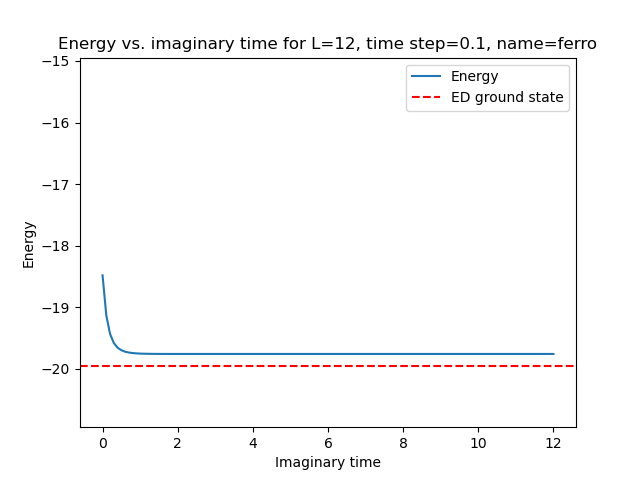
\includegraphics[width=\linewidth]{p4_1_energy_L_12time_step_0.1name_ferro.png}
  \label{fig:1a}
\end{subfigure}
\begin{subfigure}{.5\textwidth}
  \centering
  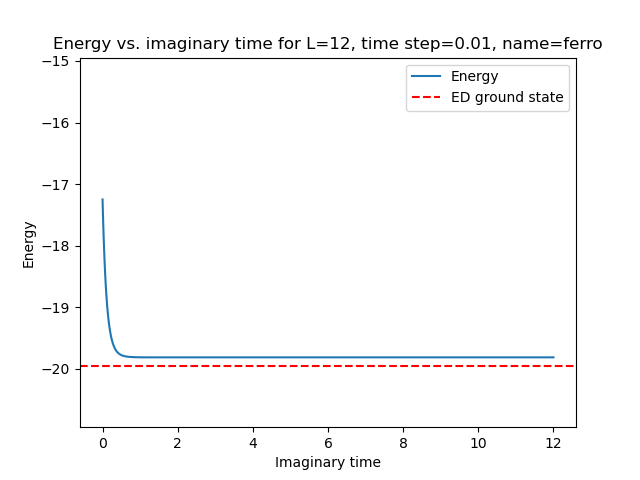
\includegraphics[width=\linewidth]{p4_1_energy_L_12time_step_0.01name_ferro.png}
  \label{fig:1b}
\end{subfigure}
\begin{subfigure}{.5\textwidth}
  \centering
  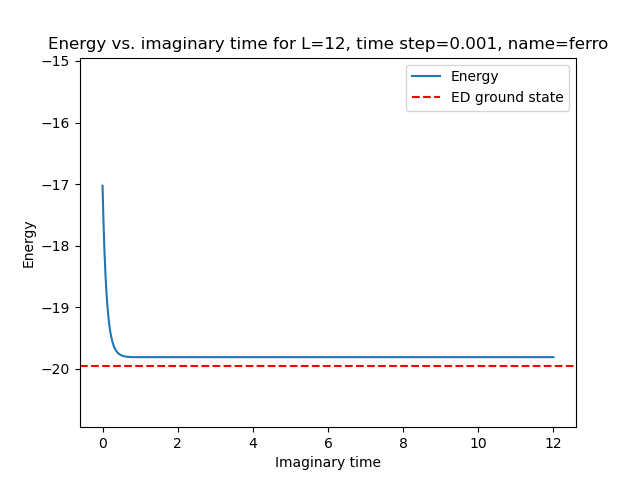
\includegraphics[width=\linewidth]{p4_1_energy_L_12time_step_0.001name_ferro.png}
  \label{fig:1c}
\end{subfigure}
\end{figure}
\begin{figure}
\begin{subfigure}{.5\textwidth}
  \centering
  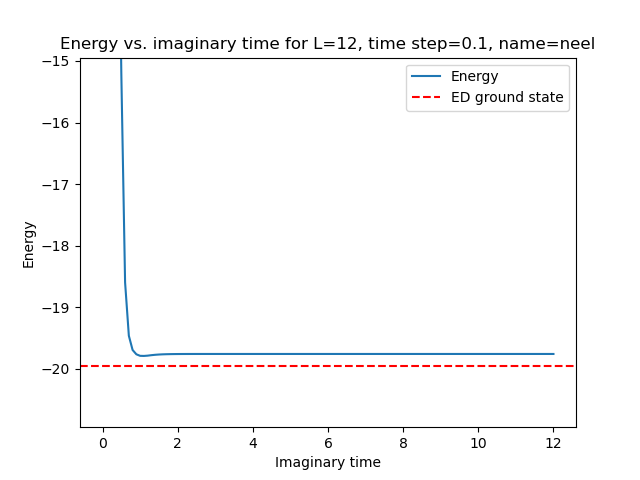
\includegraphics[width=\linewidth]{p4_1_energy_L_12time_step_0.1name_neel.png}
  \label{fig:2a}
\end{subfigure}
\begin{subfigure}{.5\textwidth}
  \centering
  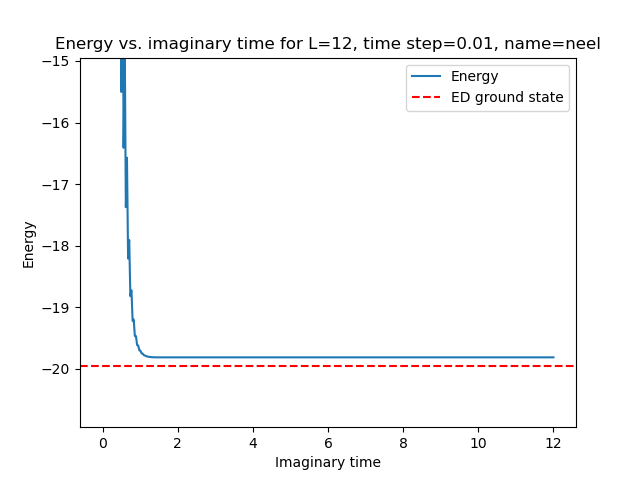
\includegraphics[width=\linewidth]{p4_1_energy_L_12time_step_0.01name_neel.png}
  \label{fig:2b}
\end{subfigure}
\begin{subfigure}{.5\textwidth}
  \centering
  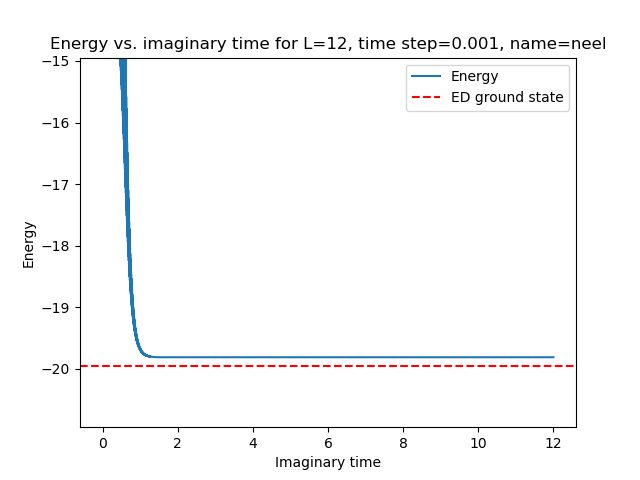
\includegraphics[width=\linewidth]{p4_1_energy_L_12time_step_0.001name_neel.png}
  \label{fig:2c}
\end{subfigure}
\end{figure}
As can be seen, an especially good approximation for the ground state is found using TEBD with imaginary time evolution. The simple ferromagnetic state is already fairly close to the ground state value, but Neel is not. For L=12, the initial trial energy was +9 for Neel, so it is noteworthy that such accurate results were able to be found at such a cheap computational cost.
\newpage

Now we no longer need to restrict to small system sizes. You can find the ground states for larger systems, like $L=32,64,128$. (If the bond dimension is kept fixed, which is suitable for ground states with finite entanglement, the computational cost grows roughly linearly with $L$ and is very manageable.) Plot the convergence of the ground state energy density, which is the extrapolation to $L \rightarrow \infty$, using the quantity $(E(L+x)-E(L)) / x$ for consecutive system sizes (you used this method in Assignment 1 to mitigate finite size effects for open boundary conditions, which is also the case here). Using the converged ground states, also measure some correlation functions in large systems.

Finally, for a fixed (large) system size, study the convergence of an initial product state with a Néel pattern $|\psi(t=0)\rangle=|\uparrow\rangle \otimes|\downarrow\rangle \otimes|\uparrow\rangle \otimes|\downarrow\rangle \otimes \cdots$, including showing the trial energy as the state cools and also measuring some correlations in the converged state. Compare to the results you found using the ferromagnetic initial state.

\subsection*{4.2 Real time evolution: quench dynamics}
Rotate back to perform real time evolution: $\tau \rightarrow i t$. The gates and MPS tensors will now generally be complex-valued, but this should require little modification to your solution from the previous\\
section. You may need to be careful here if your linear algebra routines are specialized to realvalued matrices, as you would need to switch to complex-valued routines here. If your linear algebra package figures out types automatically, you will likely not need to change the call to your diagonalization routine, but be careful to use Hermitian conjugation where required instead of matrix transpose, as these are different operations. Again choose $\delta t$ small, and use a fairly large system size $L$ (you can try multiple options). First we will study a quantum quench problem, timeevolving an arbitrary state under the Hamiltonian (15). Use the product state from the previous assignment:


\begin{equation*}
|\psi(t=0)\rangle=|\xi\rangle_{1} \otimes|\xi\rangle_{2} \otimes \cdots \otimes|\xi\rangle_{L}, \quad|\xi\rangle=\frac{1}{2}(|\uparrow\rangle-\sqrt{3}|\downarrow\rangle) \tag{23}
\end{equation*}


Encode this state as an MPS by setting the tensor components by hand. Measure some observables,

like $\left\langle\sigma_{L / 2}^{x}\right\rangle,\left\langle\sigma_{1}^{x}\right\rangle,\left\langle\sigma_{L / 2}^{z}\right\rangle$, etc., in the initial state and during the evolution. Note that the system Hamiltonian is not translation invariant because of the boundaries, and the same observables on different sites may differ at nonzero time.

Use TEBD to evolve in real time, measuring observables after every time step. Here again you may want to check your new MPS-based method against ED simulations for a small chain and short times (modifying your code from Assignment 3 to open boundary conditions), before doing more exploratory studies in what follows. Choose a maximum bond dimension (say, $\chi=16$ ) and also measure the half-system entanglement entropy $S_{L / 2}$ at every time step. You should observe that, in contrast to the imaginary-time case, the EE grows until it reaches the largest value supported by the MPS, then saturates. Once this happens we cannot trust the results of TEBD any longer; this is an important barrier to studying dynamics in large quantum systems. Repeat the experiment with larger $\chi=64,128$ and see what times you can reach with reliable results. Try a different initial state to verify that the entanglement growth is not atypical; plot all of the entanglement entropies $S_{L / 2}$ you have measured. Can you detect the saturation point (where the dynamics becomes nonphysical) in the time traces of the observables?

\subsection*{4.3 Real time evolution: TEBD projects}
The preceding section may have given you the impression that simulating real time evolution in TEBD is actually not very useful. While it's true that the linear growth of entanglement after a quench presents a challenge for any classical system-quantum architecture may be more natural for real-time simulations - there are many important applications of TEBD for real time evolution. Two are described in the optional projects below: please read through them and select at least one to study based on your interest.

\subsection*{4.3.1 Optional \#1. Quench dynamics in the MBL phase}
One very important recent application of real-time TEBD was to study dynamics in the MBL phase. Consider the Hamiltonian with random $h_{j}^{x}$ and $h_{j}^{z}$ as in Assignment 3 ; take the distributions to be of sufficient width to be deep in the MBL phase. Starting with the same product state as above, plot the time evolution of some local observables. Also plot the half-system entanglement entropy $S_{L / 2}(t)$. You will notice that it grows much more slowly than in the case with no disorder, and you can effectively go to much longer times before the entanglement becomes too large to be captured by a fixed bond dimension. By averaging over disorder realizations, attempt to characterize the MBL entanglement growth.

In fact, it was a very important finding from such a TEBD study only recently that the entanglement grows logarithmically in time as opposed to linearly in time. Careful study also finds that the entanglement entropy eventually saturates to a value proportional to the sub-system size, which was initially thought to mean that the system is not localized since this resembles the behavior of the thermalized state. However, the final value depends on the initial state and is below the expected thermal value, and it was realized that the reason for this behavior is that the simple initial state is not a locally perturbed eigenstate, so one cannot easily evaluate the localization (or lack thereof) of quantum information or energy from this quench. This led to very important insights about the MBL phase. In particular, the signature of the localization in such a quench is the logarithmic growth of $S_{L / 2}(t)$ with time, which is qualitatively distinct from ergodic (thermalizing) systems.

\subsection*{4.3.2 Optional \#2. Dynamic correlation functions}
In this part, we return to the clean system. In previous assignments, you measured correlation functions in the ground state. These are often called "static" or equal-time correlation functions. However, many important experimental probes like inelastic neutron scattering or optical conductivity are related to so-called "dynamic" correlation functions involving time evolution. For example, consider the so-called dynamic autocorrelation function for a spin at site $j$ :


\begin{equation*}
C_{j j}^{\mu \nu}(t)=\left\langle\psi_{\mathrm{gs}}\left|\sigma_{j}^{\mu}(t) \sigma_{j}^{\nu}\right| \psi_{\mathrm{gs}}\right\rangle \tag{24}
\end{equation*}


where $O(t) \equiv e^{i t H} O e^{-i t H}$ is often referred to as the "Heisenberg-evolved" operator. We work at zero temperature, so the expectation value is taken in the ground state. This can also be written


\begin{equation*}
\left.\left.C_{j j}^{\mu \nu}(t)=\left\langle\sigma_{j}^{\mu} e^{-i t H} \mid \psi_{\mathrm{gs}}\right\rangle\left|e^{-i t H} \sigma_{j}^{\nu}\right| \psi_{\mathrm{gs}}\right\rangle\right\rangle \tag{25}
\end{equation*}


The ket here is obtained by first acting with $\sigma_{j}^{\nu}$ on the ground state and then time-evolving via $e^{-i t H}$, which you can implement using TEBD. The bra is instead obtained by first time-evolving the ground state (note, which only contributes a phase!) and then acting with $\sigma_{j}^{\mu}$.

The quantum state during the time evolution in the above ket does not venture far from the ground state, as it has only finite energy and not finite energy density. Thus the time-evolved states should have low entanglement entropy and the correlation functions can be calculated for longer times than in the previous non-equilibrium quench settings. First, find the ground state $\left|\psi_{\mathrm{gs}}\right\rangle$ using imaginary-time TEBD, then use real-time TEBD to calculate $C^{z z}(t), C^{x x}(t)$, and $C^{y y}(t)$ for the site $j=L / 2$ in the middle of your system (to minimize boundary effects). Generically, such dynamical correlation functions decay exponentially in time if the system is gapped.

On the other hand, if you were to repeat this calculation for the integrable Ising chain $\left(h_{z}=0\right)$ in the gapped phase, you would find qualitatively different decay for $C^{z z}(t)$ and $C^{x x}(t)$. Repeat the experiment for this case and comment on the behavior of the time decay of correlations for integrable systems.
\footnotetext{${ }^{1}$ Bardarson, Pollmann, and Moore, PRL 109, 017202 (2012).
}


\end{document}